\documentclass[9pt,notes=hide]{beamer}
\usepackage[utf8]{inputenc}
\setbeamertemplate{navigation symbols}{}
\setbeamertemplate{caption}[numbered]
\usepackage{appendixnumberbeamer} 
\usepackage[style=authoryear, sorting=nty,backend=biber]{biblatex}
\addbibresource{Bibliography.bib}
\usetheme{Data61}
\usepackage{amsfonts}
\usepackage{datetime}
\usepackage{amsmath}
\usepackage{mcode}
\usepackage{mathtools}	
\usepackage{amssymb}
\usepackage{booktabs}
\usepackage{hyperref}
\usepackage{xcolor}
\usepackage{minted}
\usepackage{amsmath,amsthm,relsize}
\usepackage{graphicx}
\usepackage{booktabs}
\usepackage{longtable}
\usepackage{multicol}
\usepackage{multirow}

\newcommand{\linkcolor}{Data61 green}
\newcommand{\urlcolor}{Data61 dark mint}
\newcommand{\citecolor}{Data61 light forest}

\hypersetup{
  urlcolor    = \urlcolor,        %Colour for external hyperlinks
  colorlinks  = true,        %Colours links instead of ugly boxes
  linkcolor   = \linkcolor,  %Colour of internal links
  citecolor   = \citecolor   %Colour of citations
}

\makeatletter
\renewcommand*{\@textcolor}[3]{%
  \protect\leavevmode
  \begingroup
    \color#1{#2}#3%
  \endgroup
}
\makeatother
\newcommand{\vect}[1]{\boldsymbol #1}
\newcommand{\bx}{\vect{x}}
\newcommand{\by}{\vect{y}}
\newcommand{\mr}{\mathring}
\renewcommand{\geq}{\geqslant}
\renewcommand{\leq}{\leqslant}
\newcommand{\lb}{\langle}
\newcommand{\rb}{\rangle}


%Information to be included in the title page:
% New Command Maths operators
\newcommand{\bin}{\sf Bin}
\newcommand{\G}{\sf G}
\newcommand{\Hyp}{\sf Hyp}
\newcommand{\Po}{\sf Po}
\DeclareMathOperator{\logit}{logit}
\DeclareMathOperator{\expit}{expit}
\newcommand{\ex}{\sf Exp}
\newcommand{\Nor}{\sf N}
\newcommand{\gam}{\sf Gam} 
\newcommand{\Em}{\mathbb E}
\newcommand{\Pm}{\mathbb P}
\newcommand{\R}{\mathbb R}
\newcommand{\B}{\cal B}
\newcommand{\N}{\mathbb N}
\newcommand{\Z}{\mathbb Z}
\newcommand{\Q}{\mathbb Q}
\newcommand{\C}{\mathbb C}
\newcommand{\gvn}{\,|\,}
\newcommand{\e}{\mbox{e}}
\newcommand{\Var}{\mbox{Var}}
\newcommand{\cov}{\mbox{Cov}}
\newcommand{\ds}{\displaystyle}
\newcommand{\subvect}[1]{\mbox{\small \boldmath #1}}
\newcommand\isim{\stackrel{\mathclap{\normalfont\mbox{\tiny{$iid$}}}}{\sim}}
\newcommand\indsim{\stackrel{\mathclap{\normalfont\mbox{\tiny{$ind$}}}}{\sim}}

% Boldface commands and vectors
\newcommand{\vbe}{\vect{\beta}}

\newcommand{\X}{\vect{X}}
\newcommand{\Y}{\vect{Y}}
%--------------------------------------------------------------------
% Title Page
\title{Semiparametric Vector Generalized Linear Models.\\ 
    \small{Estimation and Computation}
}
\author{Gabriel Dennis}



\date{June 7, 2023}

\AtBeginSection[]
{
    \begin{frame}
        \frametitle{Table of Contents}
        \tableofcontents[currentsection]
    \end{frame}
}

\begin{document}

\maketitle

% Table of Contents 
\begin{frame}{Outline of talk}
	\tableofcontents
\end{frame}
\note[enumerate]{
}
%%%%%%%%%%%%%%%%%%%%%%%%%%%%%%%%%%%%%%%%%%%%%%%%%%


\section{Motivation}

\begin{frame}{VGLMs}
	A VGLM (Vector Generalized Linear Model)  aims to generalize GLMs to
	multivariate responses, however,  multivariate generalizations of common
	families of probability distributions (e.g., poisson, gamma, ...) are
	difficult to construct.
\end{frame}

\begin{frame}{Motivating Example (Butterfly Dataset)}
	This dataset contains $66$  counts of  $14$ species of butterflies in
	Boulder Colorado, USA. \\
	\begin{table}
		\centering
		\caption{Snippet of Butterfly Counts for the $3$ most common species \parencite{Hui2013, 2006Oliver}}
		\resizebox{0.95\textwidth}{!}{%
			\begin{tabular}{c|cccccc}
				\hline
				\textbf{site} & {\small \textbf{Pieris.rapae}} & {\small  \textbf{Colias.philodice}} & {\small \textbf{Colias.eurytheme}} & \textbf{building} & \textbf{vegetation} & \textbf{habitat} \\
				\hline
				1             & 0                              & 0                                   & 0                                  & 2.1               & 10.8                & mixed            \\
				2             & 1                              & 1                                   & 2                                  & 2.1               & 10.8                & mixed            \\
				3             & 1                              & 1                                   & 2                                  & 19.8              & 1.7                 & mixed            \\
				4             & 0                              & 2                                   & 1                                  & 5.3               & 0                   & mixed            \\
				\vdots        & \vdots                         & \vdots                              & \vdots                             & \vdots            & \vdots              & \vdots           \\
				\hline
			\end{tabular}
		}
	\end{table}
\end{frame}




\begin{frame}{Motivating Example (Butterfly Dataset)}
	Current approach is to fit independent poisson regression models for each
	species,  using geographic features of each site as covariates.\\
	\pause
	\vspace{0.1cm}\\
	We would like to fit a joint model, as species could complement or compete
	with each other within a site. \\
	\pause
	\vspace{0.1cm}\\
	However, no multivariate generalisation of the poisson distribution allows
	for both positive and negatively correlated response components.
\end{frame}




\begin{frame}
	\frametitle{Problems Modelling with parametric GLMs and VGLMs}
	Common problems that occur with parametric modelling\pause
	\begin{itemize}[<+->]
		\item requires correct specification of the error distribution
		\item requires correct specification of the mean-variance relationship
		\item observed data often exhibit over-or under-dispersion relative to the postulated model
	\end{itemize}
	\pause[\thebeamerpauses]
	For multivariate data, problems arise when specifying a parametric distribution and the response covariance structure.
	For most cases there is no standard parametric model which could produce a given dataset.
\end{frame}
\note[itemize]{
	Read the slide.
}


\section{Proposed Model}


\begin{frame}
	\frametitle{Vector Generalisation}
	This model is a vector generalisation of a Semiparametric  Generalized Linear
	Model \footnote{\parencite{Rathouz2009, Huang2012, Huang2014}}, which is
	based on a exponential tilt reformulation of the joint distribution from
	which the data originates for which  the response distribution $F$  remains
	unspecified. \\
	\pause
	\vspace{0.1cm}\\

	This allows  arbitrary nonparametric response distribution parameter $F$ and
	the  mean model parameters $\vbe$ to be simultaneously estimated without
	loss of information.

\end{frame}


\begin{frame}{Proposed Model}
	Given data
	\[
		(\Y_i, \X_i) \in \mathcal{Y} \times \mathcal{X} \subset \R^K \times \R^q, i = 1,\dots, n
	\]
	\pause
	Assume these are independent samples originating from some multivariate exponential family.
	The joint density can be written in the form
	\begin{equation*}\label{eq:referencDistribution}
		dF_i(\by) = \exp\{b_i + \vect{\theta}_i^T\by \}  \ dF(\by),  \  \ i = 1,\dots, n
	\end{equation*}
	\pause
	where $dF_i(\by)$ is an exponential tilt of the response distribution $dF(\by)$,
	with the amount of tilting $\vect{\theta}$ determined by the mean
	$\vect{\mu}(\X_i^T\vbe)$ of the observation $\Y_i$.
\end{frame}



\begin{frame}{Model Tilt Parameters}
	The normalising constants $b_i = b(\X_i, \vbe,F)$ are defined to be
	\begin{equation*}\label{eq:normalisationConstraint}
		b(\X_i, \vbe, F) = -\log \Bigg\{\int_{\mathcal{Y}} \exp\{\vect{\theta}_i^T\by \}dF(\by) \Bigg\},
	\end{equation*}
	\pause
	and the vector of tilt parameters $\vect{\theta}_i = \vect{\theta}(\X, \vbe, F) \in \R^K$ is the implicit solution to
	\begin{equation*}\label{eq:MeanConstraint}
		\mu_{(k)}(\X_{(k)}^T\vbe_{(k)}) = \int_{\mathcal{Y}}y_{(k)}\exp\{b_i + \vect{\theta}_i^T\by \}dF(\by),  \  \ k = 1,\dots,K
	\end{equation*}
\end{frame}


\begin{frame}
	\frametitle{Semiparametric Extension}
	This joint density has the log-likelihood
	\begin{equation*}\label{eq:SemiParametricLikelihood}
		\ell(\vbe, F|\X, \Y) = \sum_{i = 1}^{n} \Bigg\{ \log dF(\Y_i) + b_i + \vect{\theta}_i^T\Y_i\Bigg\}
	\end{equation*}
	\pause
	One way to estimate the densities $dF(\Y_i)$ is by replacing them  with the
	histogram estimators $p_i$, which  are assigned to values in the observed
	support $\{\Y_i \in \R^k| i = 1, 2, \dots, n \}$\\
	\pause
	\vspace{0.1cm}\\
	This produces empirical log-likelihood.
	\begin{equation*}\label{eq:chap2:empiricalLogLikelihood}
		\ell(\vbe, \vect{p}) = \sum_{i = 1}^{n} \log p_i + b_i + \vect{\theta}_i^T\Y_i
	\end{equation*}

\end{frame}


\begin{frame}
	\frametitle{Estimation of $\vbe$ and $\vect{p}$}
	$(\hat{\vbe}, \hat{\vect{p}}) $ are then the joint maximisers of the empirical log likelihood.
	\begin{equation*}
		(\hat{\vbe}, \hat{\vect{p}}) = \arg\max  \ell(\vbe, \vect{p})
	\end{equation*}
\end{frame}


\begin{frame}
	\frametitle{Estimation of $\vbe$ and $\vect{p}$}
	Subject to  empirical analogous of the normalising constraints
	\begin{equation*}\label{eq:chap2:empiricalNormalisationConstraint}
		1 = \sum_{i = 1}^{n} p_i \exp \{b_j + \vect{\theta}_j^T\Y_i \}, \  \ j = 1, 2, 3,  \dots, n
	\end{equation*}
	\pause
	and the mean constraints
	\begin{equation*}\label{eq:chap2:empiricalMeanConstraint}
		\mu_{(k)}(\X_{(k)j}^T\vbe_{(k)}) = \sum_{i = 1}^{n} p_iY_{(k)i} \exp \{b_j + \vect{\theta}_j^T\Y_i \}\  \ j = 1,  \dots, n, k = 1,\dots, K
	\end{equation*}
\end{frame}


\begin{frame}{Parameter Inference}
	There have been some results shown for the conducting parameter inference in
	the univariate case of this model \parencite{Huang2014,HuangRathouz2017},
	which generalise to this model.
\end{frame}


\begin{frame}
	\frametitle{Parameter Inference}
	For testing the null hypothesis
	\begin{align*}
		H_0:\beta_{(k)j}  & = 0,            \\
		k = 1,\dots, K, j & = 1, \dots, q_k
	\end{align*}
	\pause
	a Wald test can be used
	\begin{align*}
		\frac{\hat{\beta}_{(k)j}}{\sqrt{\hat{\Sigma}_{(k)j,(k)j}}} \sim t_{n - q_k}
	\end{align*}
	\pause
	where the standard errors are derived from the empirical log-likelihood
	\[
		\hat{\Sigma} = \Bigg\{\Var\Big[\nabla \ell (\vbe, \vect{p})\Big] \Bigg\}^{-1}
	\]
\end{frame}

\begin{frame}{Parameter Inference}
	For Point Hypothesis $H_0:\vbe = \vbe^*$
	\begin{align*}
		2\{\ell(\hat{\vbe}) - \ell(\vbe^{*}) \} \sim \chi^2_{Q},  \  \ Q = \sum_{k = 1}^{K}q_k
	\end{align*}
	\pause
	Composite Hypothesis $H_0:M\vbe = \gamma$,
	\begin{align*}
		2\{\ell(\hat{\vbe}) - \ell(\hat{\vbe}_0) \} \sim \chi^2_{r}
	\end{align*}
	\pause
	For finite samples  the following adjustment can be made
	\[
		2\{\ell(\hat{\vbe}) - \ell(\hat{\vbe}_0) \} \sim rF_{r, n - Q}
	\]
\end{frame}
\note{
	Read the slide.
}

\section{Fitting the Model}
\begin{frame}{Code}
	Currently the model is fit computationally in MATLAB using
	non-linear constrained  optimization to maximise the empirical log-likelihood.
	\footnote{The code is available at \href{https://github.com/gden173/vspglm}{github}.}
\end{frame}


\begin{frame}{Constraints}
	For $n$ observations of a $K$ dimensional response $\Y_i \in \R^K$ the optimization simultaneously solves for
	$Q + n(2 + K)$ parameters. \pause
	\begin{itemize}[<+->]
		\item  $Q$ regression parameters $\vbe$
		\item $n$ probability masses $p_i$
		\item  $n$ normalising constants $b_i$
		\item  $nK$ tilt parameters $\vect{\theta}_i$
	\end{itemize}
	\pause[\thebeamerpauses]
	which are subject to $n(K + 1)$ mean and normalising constraints.
\end{frame}



\section{Applications}

\begin{frame}{Butterfly Dataset}
	Contains $66$  counts of  $14$ species of butterfly in
	Boulder Colorado, USA. \\
	\begin{table}
		\centering
		\caption{Snippet of Butterfly Counts for the $3$ most common species}
		\resizebox{0.95\textwidth}{!}{%
			\begin{tabular}{c|cccccc}
				\hline
				site   & {\small Pieris.rapae} & {\small  Colias.philodice} & {\small Colias.eurytheme} & building & vegetation & habitat \\
				\hline
				1      & 0                     & 0                          & 0                         & 2.1      & 10.8       & mixed   \\
				2      & 1                     & 1                          & 2                         & 2.1      & 10.8       & mixed   \\
				3      & 1                     & 1                          & 2                         & 19.8     & 1.7        & mixed   \\
				4      & 0                     & 2                          & 1                         & 5.3      & 0          & mixed   \\
				\vdots & \vdots                & \vdots                     & \vdots                    & \vdots   & \vdots     & \vdots  \\
				\hline
			\end{tabular}
		}
	\end{table}
\end{frame}

\begin{frame}{Butterfly Dataset}
	We can fit this model directly to the counts of the  each  butterfly species using  separate mean models, without the need to specify any association  between species.
	\pause
	\begin{align*}
		\mu_{(k)i} & = \Em[Y_{(k)i}|\X_i] = \exp\{\X_i^T\vbe_{(k)}\}, \\
		           & i = 1, 2, \dots, 66,   \  \ k= 1,2   \dots, 14
	\end{align*}

\end{frame}

\begin{frame}[fragile]{Butterfly Dataset}
	\begin{figure}
		\centering
		\begin{verbatim}
butterfly = fit_vspglm(...
         ["colias.philodice ~ (building,urban,habitat)",...
         "pieris.rapae ~ (building, urban, habitat)", ...
         "colias.eurytheme ~ (building, urban, habitat)"], ...
         tbl, {'log', 'log', 'log'})
\end{verbatim}
		\caption{Formula Syntax to fit $3$ separate unconstrained models using the same covariates and log link functions}
	\end{figure}
\end{frame}

\note[itemize]{
	\item This next example shows this models applicability to an almost arbitrary number of response components.
	\item Read Slide}
\begin{frame}{Butterfly Dataset}
	\begin{figure}
		\centering
		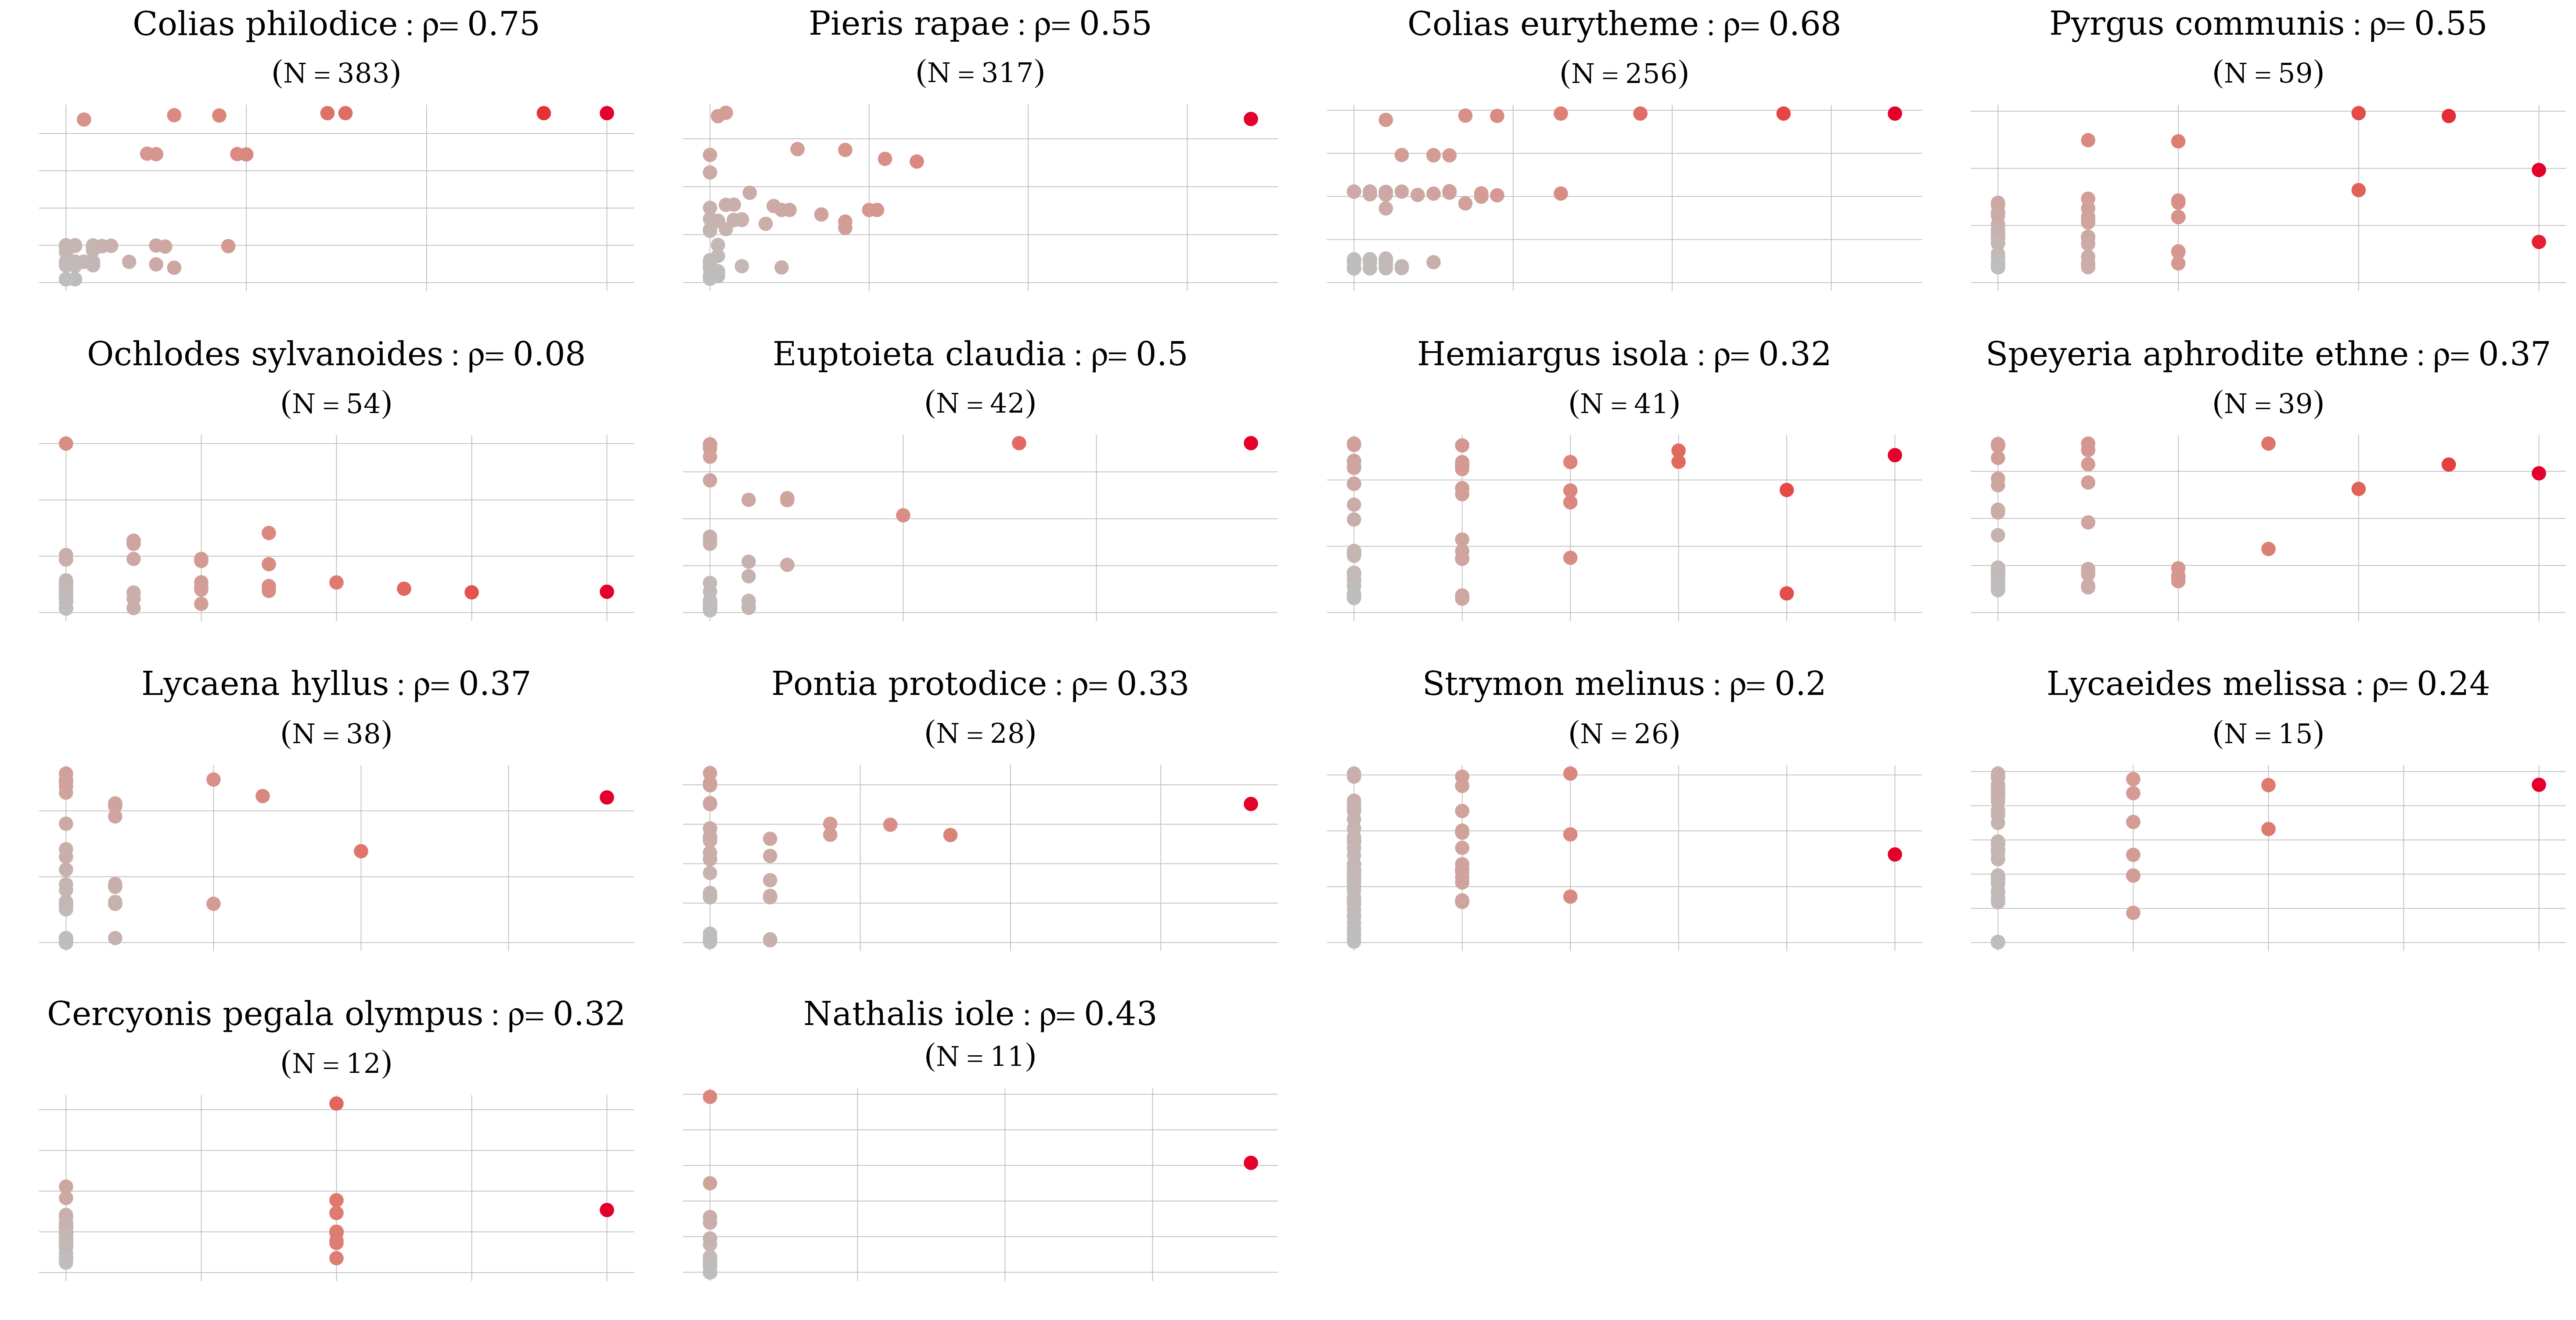
\includegraphics[width = 0.9\textwidth]{figures/butterfly_14d_poisson.png}
		\caption{Predictions ($y$-axis) vs Observed counts ($x$-axis) }
		\label{fig:butterfly_14d}
	\end{figure}
\end{frame}

\begin{frame}{Butterfly Dataset}
	\begin{figure}
		\centering
		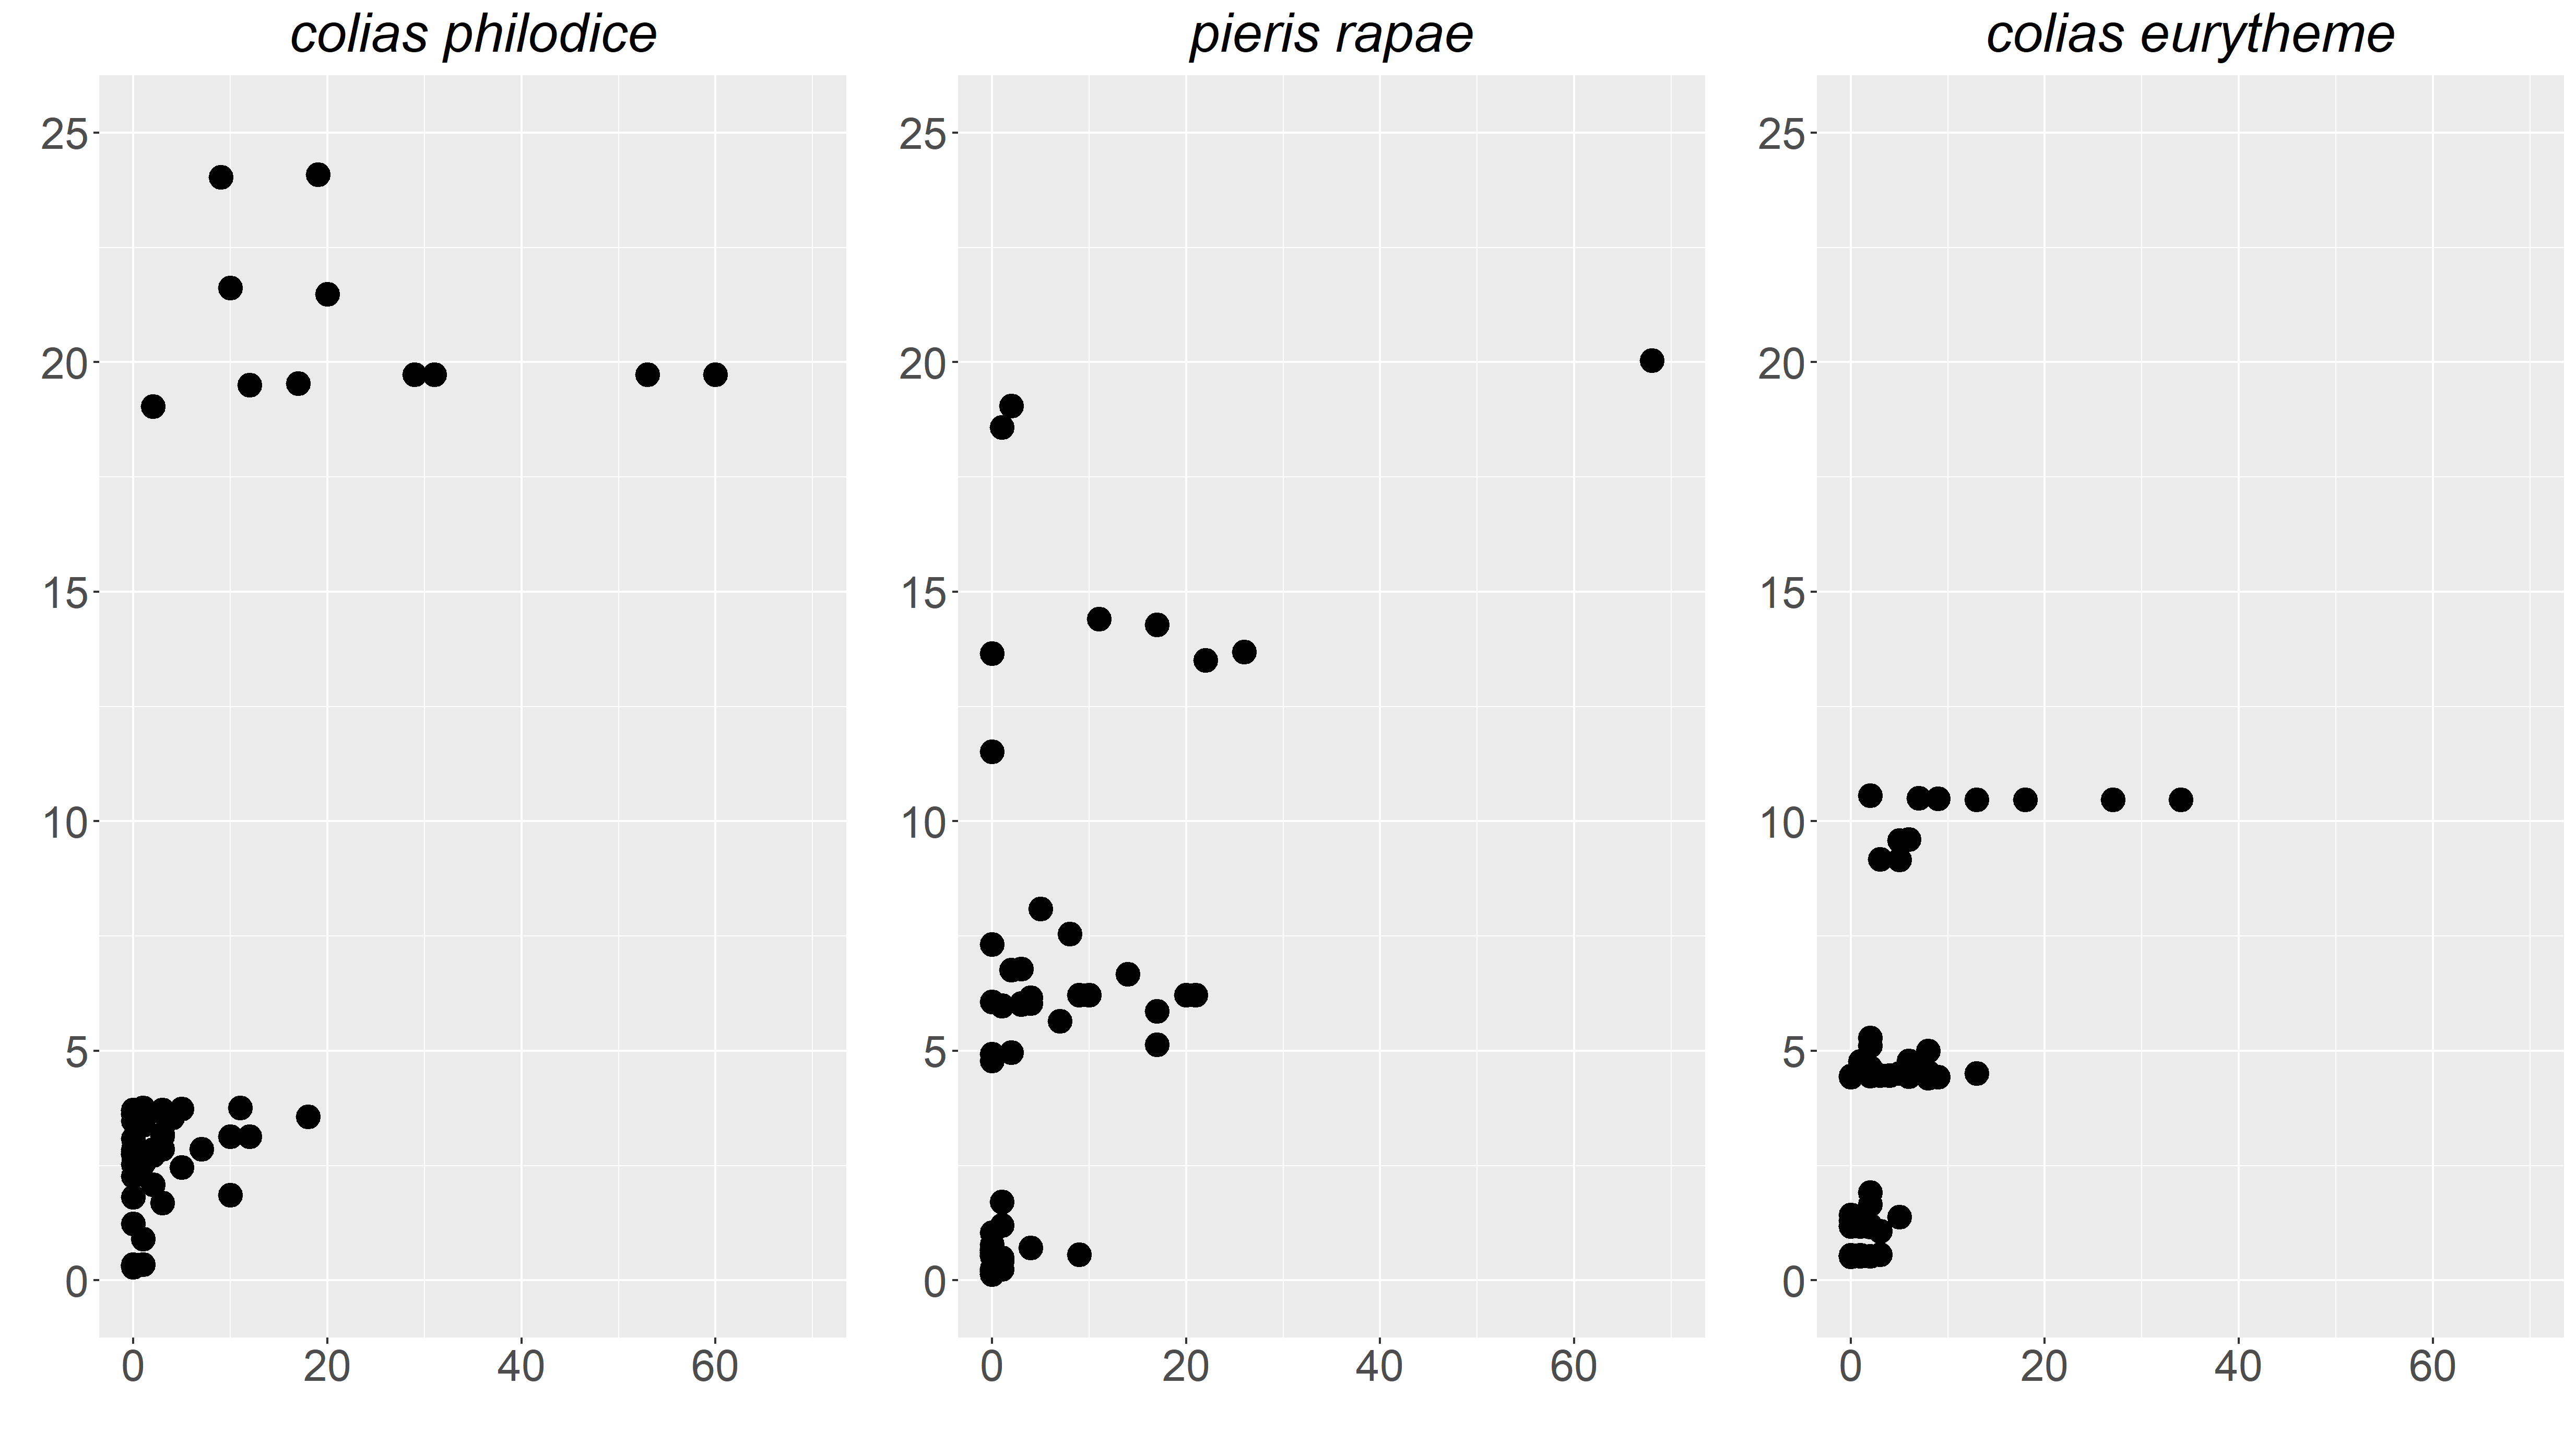
\includegraphics[width = \textwidth]{figures/butterfly_3d_poisson.png}
		\caption{Predictions ($y$-axis) vs Observed counts ($x$-axis) for the $3$ butterfly species with the greatest number of observed counts}
		\label{fig:butterfly_3d}
	\end{figure}
\end{frame}



\begin{frame}{Burns Injury Dataset}
	Contains $981$ observations of patients admitted to hospital with 3rd degree burns.
	\begin{table}
		\centering
		\caption{Snippet of Burns Dataset \parencite{}}
		\begin{tabular}{lccc}
			\hline
			{}     & \textbf{age} & \textbf{burns} & \textbf{death} \\ \hline
			1      & 3            & 6.9            & 1              \\
			2      & 39           & 7.4            & 1              \\
			3      & 42           & 3.9            & 1              \\
			4      & 21           & 6.1            & 1              \\
			\vdots & \vdots       & \vdots         & \vdots         \\
			\hline
		\end{tabular}
	\end{table}
\end{frame}

\begin{frame}[fragile]{Burns Injury Data Set}
	Response vector has two components $\Y = (Y_{\text{death}}, Y_{\text{burn}})$ , which are binary and continuous,  and a single covariate $\X = (X_{\text{age}})$.\\
	\pause
	This suggests the two marginal mean models
	\begin{align*}
		\mu_{(1)} = \Em[\text{death}|\text{age}] & =  \frac{\exp\{\beta_{(1)1} + \beta_{(1)2}\text{age}\}}{1 + \exp\{\beta_{(1)1} +\beta_{(1)2}\text{age}\}} \\
		\mu_{(2)} = \Em[\text{burns}|\text{age}] & = \beta_{(2)1} + \beta_{(2)2}\text{age}
	\end{align*}
	\pause
	\vspace{0.2cm}\\
	The code for fitting this model is
	\begin{verbatim}
model = fit_vspglm(["death~age","burns~age"],tbl,{'logit','id'})
\end{verbatim}

\end{frame}



\begin{frame}{Burn Injury Data Set}
	This data set has been analysed several times using a variety of VGLMS,
	with \textcite{Huang2017}  using GEEs to fit these mean models.\\
	\vspace{0.5cm}\\
	\pause
	GEE model parameters
	\begin{align*}
		\hat{\mu}_{(1)} & = \frac{\exp\{-3.6891 + 0.0508\text{age}\}}{1 + \exp\{-3.6891 + 0.0508\text{age}\}} \\
		\hat{\mu}_{(2)} & =  6.7118 + 0.0035\text{age} \nonumber
	\end{align*}
	\pause
	VSPGLM model parameters
	\begin{align*}
		\hat{\mu}_{(1)} & = \frac{\exp\{-3.657  + 0.0509\text{age}\}}{1 + \exp\{-3.657  + 0.0509\text{age}\}} \\
		\hat{\mu}_{(2)} & =  6.7318 + 0.0027\text{age} \nonumber
	\end{align*}
\end{frame}

\begin{frame}{Burn Injury Data Set}
	\begin{table}[h!]
		\centering
		\begin{tabular}{c|c}
			{}                                 & $\text{se}(\hat{\vbe})$ \\
			\hline
			$\beta_{\text{death}, \text{age}}$ & 0.0051                  \\
			$\beta_{\text{burns}, \text{age}}$ & 0.0017
		\end{tabular}
		\caption{GEE corrected standard errors}
		\label{tab:GEEerrors}
	\end{table}
	\begin{table}[h!]
		\centering
		\begin{tabular}{c|c}
			{}                                 & $\text{se}(\hat{\vbe}$) \\
				\hline
			$\beta_{\text{death}, \text{age}}$ & 0.0045                  \\
			$\beta_{\text{burns}, \text{age}}$ & 0.0019
		\end{tabular}
		\caption{VSPGLM standard errors}
		\label{tab:VSPGLMerrors}
	\end{table}
\end{frame}


\begin{frame}{Sorbinil Dataset}
	Contains $n = 41$ observations of itching scores $(Y_L, Y_R)$ for the
	left and right eye after the application of sorbinil or a placebo,
	measured on a $9$ point Likert scale between $0$ and $4$ with increments of $0.5$. \\
	\begin{table}
		\centering
		\caption{Snippet of Sorbinil dataset \parencite{Rosner2006}}
		\resizebox{0.95\textwidth}{!}{%
			\begin{tabular}{ll|ll|ll|ll}
				\toprule
				\multicolumn{2}{c}{$n = 6$} & \multicolumn{2}{c}{$n = 14$} & \multicolumn{2}{c}{$n = 14$} & \multicolumn{2}{c}{$n = 7$}                                                                              \\
				\textbf{Sorbinil}           & \textbf{Sorbinil}            & \textbf{Sorbinil}            & \textbf{Placebo}            & \textbf{Placebo} & \textbf{Sorbinil} & \textbf{Placebo} & \textbf{Placebo} \\
				\textbf{Left}               & \textbf{Right}               & \textbf{Left}                & \textbf{Right}              & \textbf{Left}    & \textbf{Right}    & \textbf{Left}    & \textbf{Right}   \\ \toprule
				2                           & 2                            & 1                            & 1.5                         & 2.5              & 2                 & 3                & 3                \\
				1                           & 1                            & 2                            & 2.5                         & 2.5              & 2.5               & 2                & 3                \\
				0.5                         & 2                            & 3                            & 1                           & 3                & 3                 & 2.5              & 2.5              \\
				\vdots                      & \vdots                       & \vdots                       & \vdots                      & \vdots           & \vdots            & \vdots           & \vdots           \\
			\end{tabular}
		}
	\end{table}
\end{frame}


\begin{frame}[fragile]{Sorbinil Dataset}
	We would like to see if sorbinil has a significant effect in reducing\\  
        itching scores for each eye.
	\vspace{0.3cm}\\
	\pause
        Previous attempts at modeling this dataset using VGLMs standardise
        these scores to $[0,1]$ and fit logistic mean models,
	however, this is  unnecessary when using this model. \\
	\pause
	\vspace{0.1cm}\\
	The following symmetric model was found to be adequate
	\[
		\mu_L = \beta_0 + \beta_1 \mathcal{I}_L,  \  \ \mu_R = \beta_0 + \beta_1 \mathcal{I}_R
	\]

	\pause
	This model finds  a significant effect that sorbinil reduces itching scores by $0.43$.\\
	\pause
	\vspace{0.5cm}\\
	The code to fit this symmetric model is
	\begin{verbatim}
    sorbinil = fit_vspglm(["(Y_L, Y_R) ~ (I_L & I_R)"], tbl, {'id'})
 \end{verbatim}
\end{frame}


\begin{frame}{Sorbinil Dataset}
	\begin{figure}
		\centering
		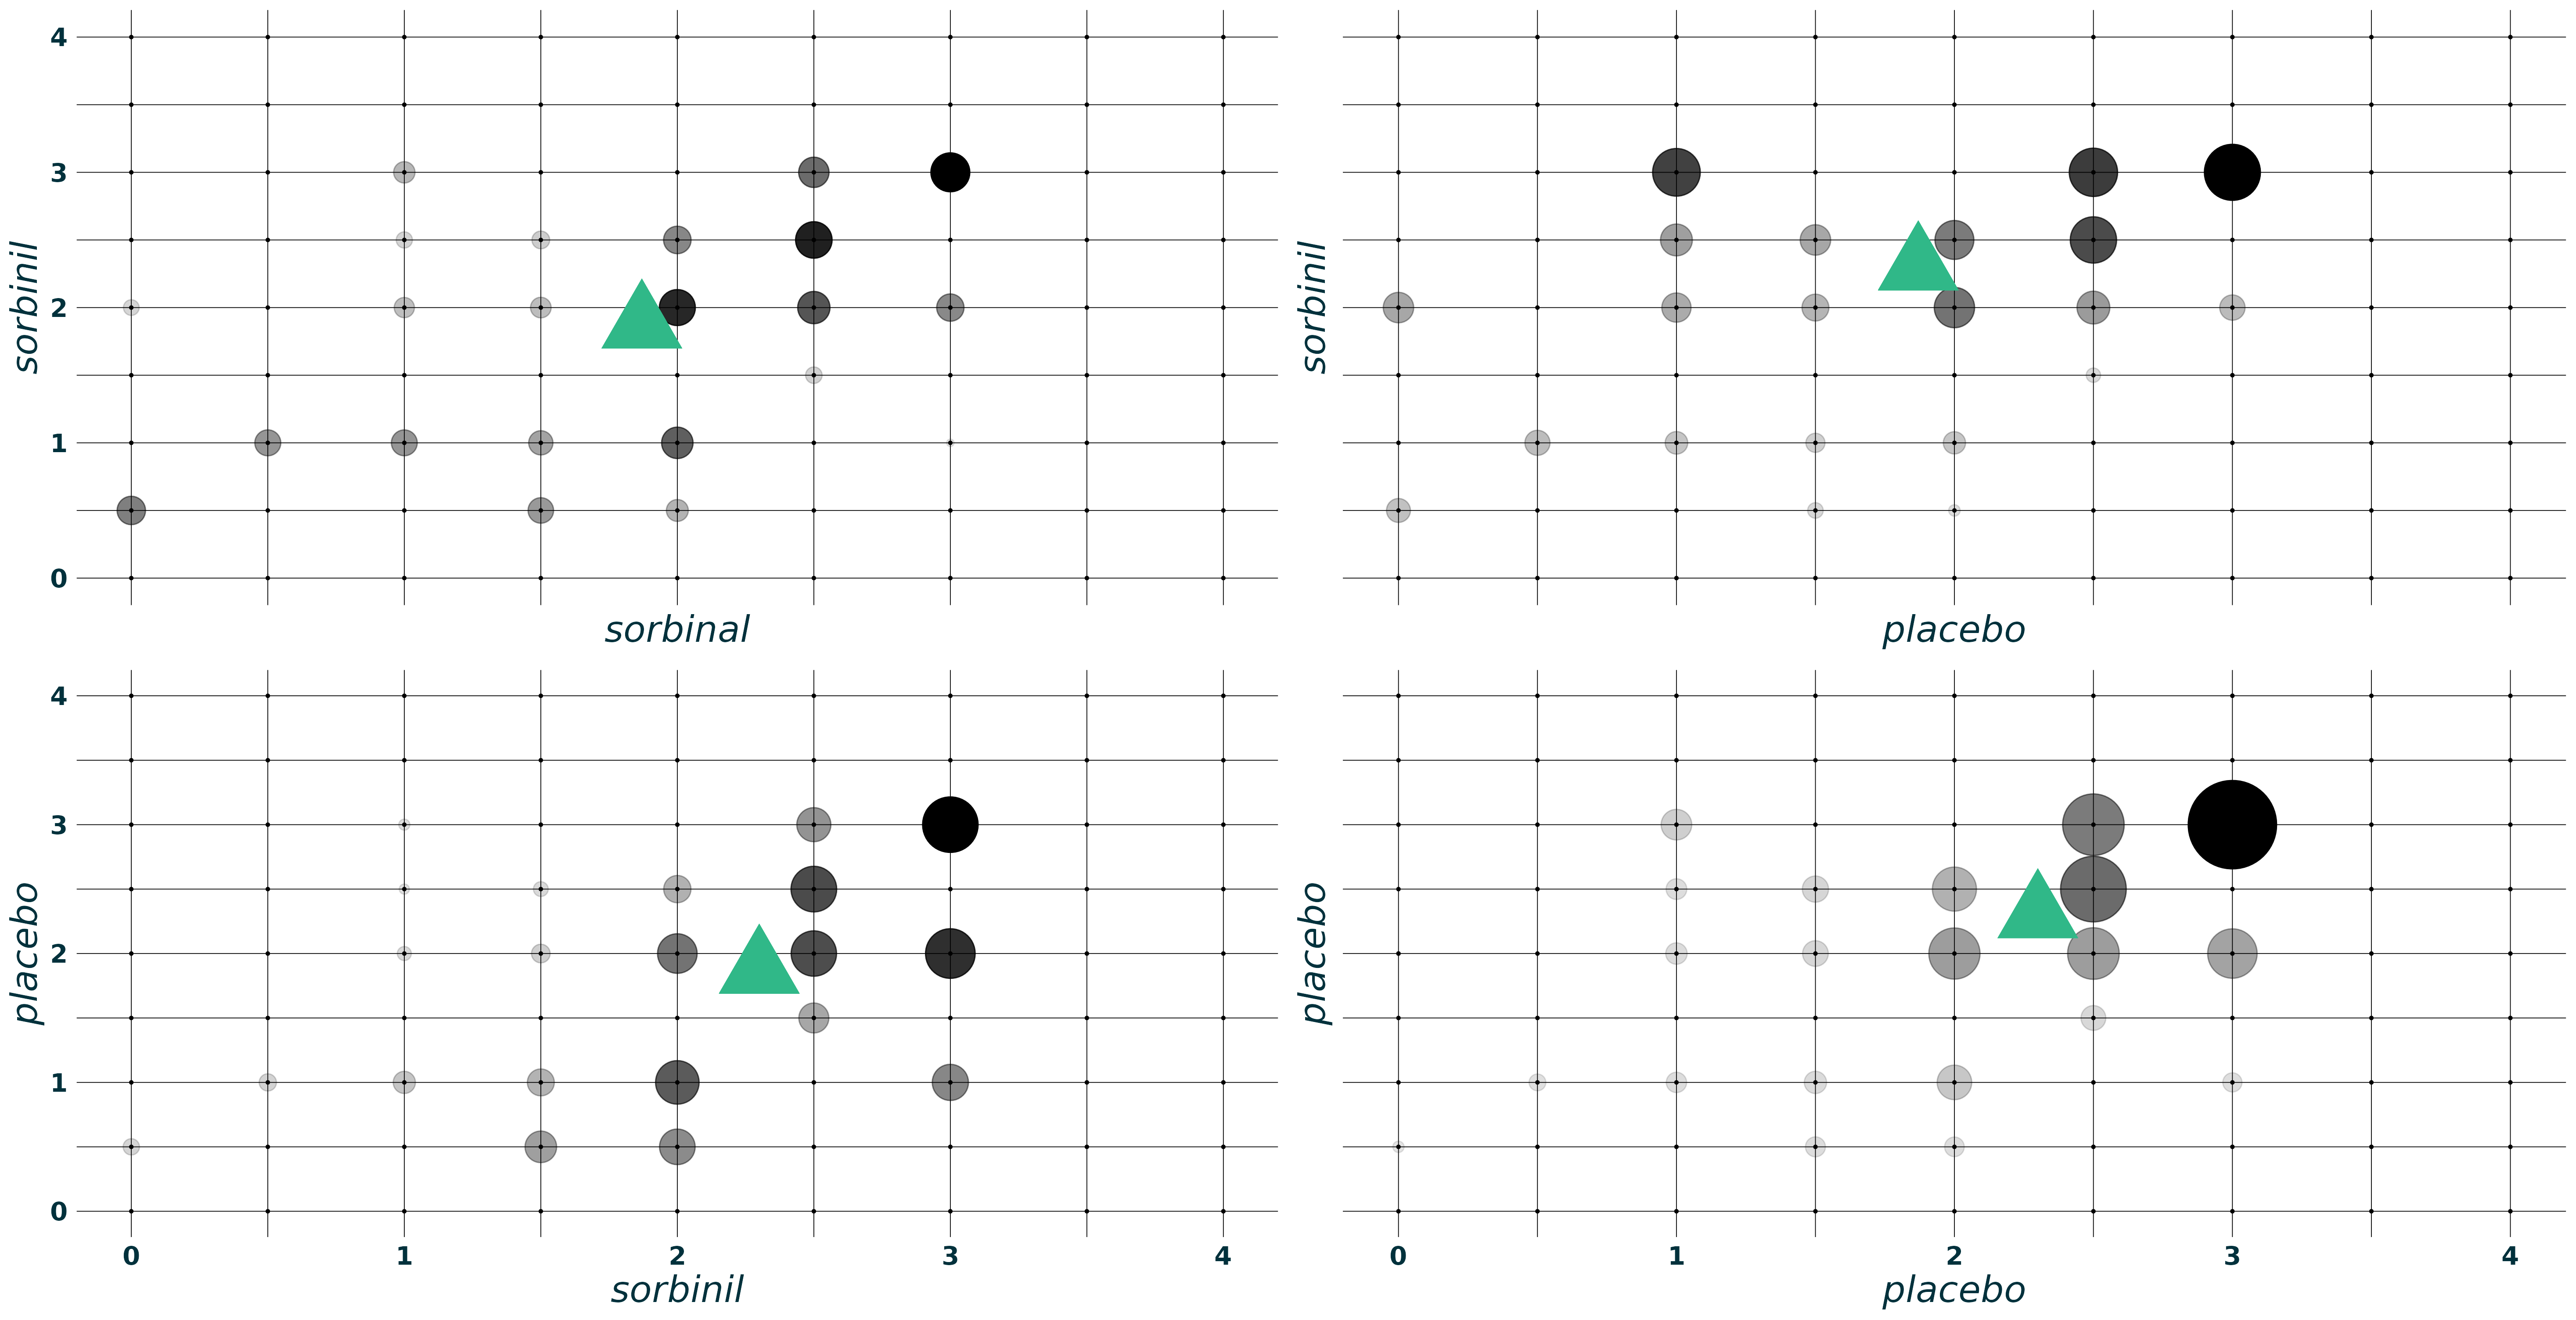
\includegraphics[width= \linewidth]{figures/sorbinil_pmfs.png}
		\caption{{\small Reweighted Sorbinal pmf at group medians (left eye = $y$ axis, right eye = $x$ axis)}}
	\end{figure}
\end{frame}


\begin{frame}[allowframebreaks]
	\frametitle{Bibliography}
	\printbibliography
\end{frame}

\appendix

\begin{frame}{Trivariate Poisson Model}
	\begin{align*}
		\alpha               & \sim  \mathcal{N}(0, \sigma_{0}^2),  \  \ \sigma \in \R_+ \nonumber  \\
		\X                   & \sim   \ {\sf U}[-1, 1]^3  \nonumber                                 \\
		Y_1|\alpha, \X_{(1)} & \sim \text{Pois}(\exp(\X_{(1)}^T\vbe_{(1)} + \alpha))  \nonumber     \\
		Y_2|\alpha, \X_{(2)} & \sim  \text{Pois}(\exp(\X_{(2)}^T\vbe_{(2)} + 0.5\alpha))            \\
		Y_3|\alpha, \X_{(3)} & \sim  \text{Pois}(\exp(\X_{(3)}^T\vbe_{(3)} - 0.3\alpha))  \nonumber
	\end{align*}
\end{frame}

\begin{frame}{Trivariate  Poisson Simulation Results }
	\begin{table}
		\centering
		\caption{Simulation results for trivariate Poisson  model using a sample size of $n = 200$ and $N = 1000$ simulations}
		\resizebox{\textwidth}{!}{%
			\begin{tabular}{@{}lllllclll@{}}
				\toprule
				\multirow{2}{*}[-1em]{$\vbe$} & \multirow{2}{*}[-1em]{$\hat{\vbe}$} & \multirow{2}{*}[-1em]{$|\vbe - \hat{\vbe}|$ } & \multicolumn{2}{c}{Errors} & \multirow{2}{*}[-1em]{$p \leq 0.05$} & \multicolumn{3}{c}{CI}                            \\
				\addlinespace[10pt]
				\cmidrule(lr){4-5} \cmidrule(lr){7-9}                                                                                                                                                                                                       \\
				{}                            & {}                                  & {}                                            & $\hat{\sigma}$             & $\bar{\text{se}}(\hat{\vbe})$        & {}                     & $90\%$ & $95\%$ & $99\%$ \\
				\midrule
				0.4                           & 0.40                                & 0.004                                         & 0.13                       & 0.12                                 & 0.88                   & 0.89   & 0.94   & 0.99   \\
				-0.8                          & -0.79                               & 0.002                                         & 0.13                       & 0.14                                 & 0.99                   & 0.93   & 0.96   & 0.99   \\
				0                             & 0.001                               & 0.001                                         & 0.13                       & 0.12                                 & 0.05                   & 0.89   & 0.95   & 0.99   \\
				\bottomrule
			\end{tabular}

		}
	\end{table}
\end{frame}


\begin{frame}{Trivariate Mixed Effects Simulation}
	\begin{align*}
		\alpha                & \sim  \  \mathcal{N}(0,  \ \sigma_0^2)\nonumber                                     \\
		\X                    & \sim   \ {\sf U}[-1, 1]^3  \nonumber                                                \\
		\Y_1|\X_{(1)}, \alpha & \sim  \  \mathcal{N}(\X_{(1)}^T\vbe_{(1)} + \alpha,  \ \sigma_1^2)                  \\
		\Y_2|\X_{(2)}, \alpha & \sim   \ {\sf Pois}(\exp(\X_{(2)}^T\vbe_{(2)}  + 0.5\alpha))\nonumber               \\
		\Y_3|\X_{(3)}, \alpha & \sim  \ {\sf Gamma}(\lambda, \  \exp(\X_{(3)}^T\vbe_{(3)}   - 0.3\alpha)) \nonumber
	\end{align*}
\end{frame}


\begin{frame}{Trivariate Mixed Effects Simulation Results }
	\begin{table}
		\centering
		\caption{Simulation results for trivariate mixed effects model using a sample size of $n = 200$ and $N = 1000$ simulations}
		\resizebox{\textwidth}{!}{%
			\begin{tabular}{@{}llllllclll@{}}
				\toprule
				\multirow{2}{*}[-1em]{Margin} & \multirow{2}{*}[-1em]{$\vbe$} & \multirow{2}{*}[-1em]{$\hat{\vbe}$} & \multirow{2}{*}[-1em]{$|\vbe - \hat{\vbe}|$ } & \multicolumn{2}{c}{Errors} & \multirow{2}{*}[-1em]{$p \leq 0.05$} & \multicolumn{3}{c}{CI}                            \\
				\addlinespace[10pt]
				\cmidrule(lr){5-6} \cmidrule(lr){8-10}                                                                                                                                                                                                                                      \\
				{}                            & {}                            & {}                                  & {}                                            & $\hat{\sigma}$             & $\bar{\text{se}}(\hat{\vbe})$        & {}                     & $90\%$ & $95\%$ & $99\%$ \\
				\midrule
				Normal                        & 1                             & 1.005                               & 0.0058                                        & 0.17                       & 0.18                                 & 1                      & 0.90   & 0.95   & 0.99   \\
				Poisson                       & -0.5                          & -0.49                               & 0.0005                                        & 0.13                       & 0.13                                 & 0.96                   & 0.83   & 0.88   & 0.93   \\
				Gamma                         & 0.4                           & 0.39                                & 0.004                                         & 0.12                       & 0.13                                 & 0.85                   & 0.89   & 0.93   & 0.97   \\
				\bottomrule
			\end{tabular}
		}
	\end{table}
\end{frame}

\begin{frame}{Multivariate Normal Simulation Results}
	\begin{table}
		\centering
		\caption{Simulation results for bivariate normal model using  sample size of $n = 200$ and $N = 1000$ simulations}
		\resizebox{\textwidth}{!}{%
			\begin{tabular}{@{}lllllclll@{}}
				\toprule
				\multirow{2}{*}[-1em]{$\vbe$} & \multirow{2}{*}[-1em]{$\hat{\vbe}$} & \multirow{2}{*}[-1em]{$|\vbe - \hat{\vbe}|$ } & \multicolumn{2}{c}{Errors} & \multirow{2}{*}[-1em]{$p \leq 0.05$} & \multicolumn{3}{c}{CI}                            \\
				\addlinespace[10pt]
				\cmidrule(lr){4-5} \cmidrule(lr){7-9}                                                                                                                                                                                                       \\
				{}                            & {}                                  & {}                                            & $\hat{\sigma}$             & $\bar{\text{se}}(\hat{\vbe})$        & {}                     & $90\%$ & $95\%$ & $99\%$ \\
				\midrule
				-1                            & -0.99                               & 0.0004                                        & 0.11                       & 0.11                                 & 1                      & 0.91   & 0.95   & 0.99   \\
				0                             & -0.0004                             & 0.0004                                        & 0.11                       & 0.11                                 & 0.05                   & 0.90   & 0.95   & 0.99   \\
				0.5                           & 0.49                                & 0.009                                         & 0.14                       & 0.13                                 & 0.95                   & 0.88   & 0.94   & 0.98   \\
				2.2                           & 2.19                                & 0.003                                         & 0.14                       & 0.14                                 & 1                      & 0.90   & 0.94   & 0.98   \\
				\bottomrule
			\end{tabular}
		}
	\end{table}
\end{frame}


\begin{frame}{$F$ simulation results}
	\begin{table}[H]
		\centering
		\caption{Type \rom{1} errors at significance levels of $0.10, 0.05$ and $0.01$ using  sample sizes of $n = 75, 150$, and $N = 3000$ simulations}
		\begin{tabular}{@{}l|lll@{}}
			\toprule
			{}  & \multicolumn{3}{c}{Type \rom{1} Errors}                   \\
			$n$ & $0.10$                                  & $0.05$ & $0.01$ \\
			\midrule
			75  & 0.119                                   & 0.060  & 0.012  \\
			150 & 0.097                                   & 0.050  & 0.013  \\
			\bottomrule
		\end{tabular}
	\end{table}
\end{frame}
\end{document}








